
\documentclass[a4paper,12pt]{article}
%%%%%%%%%%%%%%%%%%%%%%%%%%%%%%%%%%%%%%%%%%%%%%%%%%%%%%%%%%%%%%%%%%%%%%%%%%%%%%%%%%%%%%%%%%%%%%%%%%%%%%%%%%%%%%%%%%%%%%%%%%%%%%%%%%%%%%%%%%%%%%%%%%%%%%%%%%%%%%%%%%%%%%%%%%%%%%%%%%%%%%%%%%%%%%%%%%%%%%%%%%%%%%%%%%%%%%%%%%%%%%%%%%%%%%%%%%%%%%%%%%%%%%%%%%%%
\usepackage{eurosym}
\usepackage{vmargin}
\usepackage{amsmath}
\usepackage{graphics}
\usepackage{epsfig}
\usepackage{subfigure}
\usepackage{fancyhdr}
\usepackage{listings}
\usepackage{framed}
\usepackage{graphicx}

\setcounter{MaxMatrixCols}{10}
%TCIDATA{OutputFilter=LATEX.DLL}
%TCIDATA{Version=5.00.0.2570}
%TCIDATA{<META NAME="SaveForMode" CONTENT="1">}
%TCIDATA{LastRevised=Wednesday, February 23, 2011 13:24:34}
%TCIDATA{<META NAME="GraphicsSave" CONTENT="32">}
%TCIDATA{Language=American English}

\pagestyle{fancy}
\setmarginsrb{20mm}{0mm}{20mm}{25mm}{12mm}{11mm}{0mm}{11mm}
\lhead{MA4128} \rhead{Mr. Kevin O'Brien}
\chead{Principal Component Analysis}
%\input{tcilatex}

\begin{document}
	
	\tableofcontents
	%http://support.sas.com/publishing/pubcat/chaps/55129.pdf

%--------------------------------------------------------------------------------------------------%
\section{Exploratory Factor Analysis}
Principal Component Analysis (PCA) and Exploratory Factor Analysis (EFA) are both variable reduction techniques
and sometimes mistaken as the same statistical method. However, there are distinct differences between PCA and
EFA. Similarities and differences between PCA and EFA will be examined.


\subsection{Principal Component Analysis (PCA)}
\begin{itemize}
\item Is a variable reduction technique
\item Is used when variables are highly correlated
\item Reduces the number of observed variables to a smaller number of principal components which account for most
of the variance of the observed variables
\item Is a large sample procedure
\end{itemize}

The number of components extracted is equal to the number of observed variables in the analysis. The first principal
component identified accounts for most of the variance in the data. The second component identified accounts for the
second largest amount of variance in the data and is uncorrelated with the first principal component and so on.


The total amount of variance in PCA is equal to the number of observed variables being analyzed. In PCA, observed
variables are standardized, (e.g., mean=0, standard deviation=1).

Components accounting for maximal variance are retained while other components accounting for a trivial amount of
variance are not retained. Eigenvalues indicate the amount of variance explained by each component. Eigenvectors
are the weights used to calculate components scores.


\subsection{Factor Analysis}
Factor analysis is a statistical procedure to identify interrelationships that
exist among a large number of variables, i.e.,  to identify how suites of
variables are related.

Factor analysis can be used for exploratory or confirmatory purposes.
As an exploratory procedure, factor analysis is used to search for a
possible underlying structure in the variables. In confirmatory research,
the researcher evaluates how similar the actual structure of the data, as
indicated by factor analysis, is to the expected structure.

The major difference between exploratory and confirmatory factor
analysis is that researcher has formulated hypotheses about the
underlying structure of the variables when using factor analysis for
confirmatory purposes.

As an exploratory tool, factor analysis doesn't have many statistical
assumptions. The only real assumption is presence of relatedness
between the variables as represented by the correlation coefficient. If
there are no correlations, then there is no underlying structure.

\subsection{Exploratory Factor Analysis (EFA)}
\begin{itemize}
\item Is a variable reduction technique which identifies the number of \textbf{\emph{latent constructs}} and the underlying factor
structure of a set of variables
\item Hypothesizes an underlying construct, a variable not measured directly
\item Estimates factors which influence responses on observed variables
\item Allows you to describe and identify the number of latent constructs (also known as factors)
\item Includes unique factors, error due to unreliability in measurement
\item Traditionally has been used to explore the possible underlying factor structure of a set of measured variables without imposing any preconceived structure on the outcome.
\end{itemize}

The figure below shows four \textbf{\emph{factors}} (ovals) each measured by 3 observed variables (rectangles) with unique factors. Since measurement is not perfect, error or unreliability is estimated and specified explicitly in the diagram.

\textbf{\emph{Factor loadings}} (parameter estimates) help interpret factors. Loadings are the correlation between observed variables and factors, are standardized regression weights if variables are standardized (weights used to predict variables from factor). Standardized linear weights represent the effect size of the factor
on variability of observed variables.

\begin{figure}[h!]
\begin{center}
  % Requires \usepackage{graphicx}
  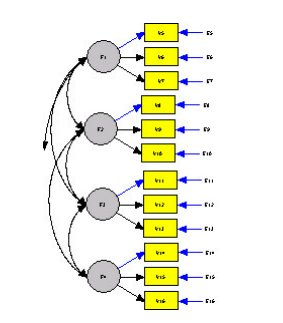
\includegraphics[scale=0.6]{4AFactor.jpg}\\
  \caption{Factor Analysis}
\end{center}
\end{figure}

In Exploratory Factor Analysis, observed variables are a linear combination of the underlying factors (estimated factor and a unique factor).

Communality is the variance of observed variables accounted for by a common factor. Large communality is strongly
influenced by an underlying construct.

\subsection{Similarities between PCA and EFA}
\begin{itemize}
\item PCA and EFA have these assumptions in common:
\begin{itemize}
\item Measurement scale is interval or ratio level
\item Random sample - at least 5 observations per observed variable and at least 100 observations.
\item Larger sample sizes recommended for more stable estimates, 10-20 observations per observed variable
\end{itemize}
\item `Over-sample' to compensate for missing values
\item Linear relationship between observed variables
\item Normal distribution for each observed variable
\item Each pair of observed variables has a bivariate normal distribution
\item PCA and EFA are both variable reduction techniques. (If communalities are large, close to 1.00, results could be similar.)
\end{itemize}

\subsection{Differences between PCA and FA}
These techniques are typically used to analyze groups of correlated variables representing one or more common domains; for example, indicators of socioeconomic status, job satisfaction, health, self-esteem, political attitudes or family values. 
Principal components analysis is used to find optimal ways of combining variables into a small number of subsets, while factor analysis may be used to identify the structure underlying such variables and to estimate scores to measure latent factors themselves. The main applications of these techniques can be found in the analysis of multiple indicators, measurement and validation of complex constructs, index and scale construction, and data reduction. These approaches are particularly useful in situations where the dimensionality of data and its structural composition are not well known.

When an investigator has a set of hypotheses that form the conceptual basis for her/his factor analysis, the investigator performs a confirmatory, or hypothesis testing, factor analysis. In contrast, when there are no guiding hypotheses, when the question is simply what are the underlying factors the investigator conducts an exploratory factor analysis. 

The factors in factor analysis are conceptualized as "real world" entities such as depression, anxiety, and disturbed thought. This is in contrast to principal components analysis (PCA), where the components are simply geometrical abstractions that may not map easily onto real world phenomena.

\subsubsection{ Treatment of Variance}

Another difference between the two approaches has to do with the variance that is analyzed. In PCA, all of the observed variance is analyzed, while in factor analysis it is only the shared variances that is analyzed.
\begin{itemize}
\item Principal Components retained account for a maximal amount of variance of observed variables.
Factors account for common variance in the data.

\item PCA Analysis decomposes correlation matrix. EFA  decomposes adjusted correlation matrix.

\item PCA: Ones on the diagonals of the correlation matrix. EFA Diagonals of correlation matrix adjusted with unique factors.

\item PCA: Minimizes sum of squared perpendicular distance to
the component axis. EFA: Estimates factors which influence responses on
observed variables.
\item PCA: Component scores are a linear combination of the
observed variables weighted by eigenvectors.
EFA: Observed variables are linear combinations of the
underlying and unique factors.
\end{itemize}


%---------------------------------------------------------------------------------------------%
\newpage

\subsection{PCA Terminology}
\begin{itemize}
\item  PC loadings are correlation coefficients between the PC scores and the
original variables.
\item  PC loadings measure the importance of each variable in accounting for the
variability in the PC.  It is possible to interpret the first few PCs in terms of
'overall' effect or a 'contrast' between groups of variables based on the
structures of PC loadings.
\item high correlation between PC1 and a variable indicates that the variable is
associated with the direction of the maximum amount of variation in the
dataset.
\item More than one variable might have a high correlation with PC1. A strong
correlation between a variable and PC2 indicates that the variable is
responsible for the next largest variation in the data perpendicular to PC1,
and so on.
\item  if a variable does not correlate to any PC, or correlates only with the last PC,
or one before the last PC, this usually suggests that the variable has little or
no contribution to the variation in the dataset. Therefore, PCA may often
indicate which variables in a dataset are important and which ones may be of
little consequence. Some of these low-performance variables might
therefore be removed from consideration in order to simplify the overall
analyses.
\end{itemize}


\subsection{Communality} 
Communality refers to the total amount of variance an original variable shares with all other
variables included in the analysis.This is the proportion of each variable's variance that can be explained by the principal components .  (It is denoted as $h^2$ and can be defined as the sum of squared factor loadings).

\textbf{Initial} - By definition, the initial value of the communality in a principal components analysis is 1.

\textbf{Extraction}  - The values in this column indicate the proportion of each variable's variance that can be explained by the principal components.  Variables with high values are well represented in the common factor space, while variables with low values are not well represented. They are the reproduced variances from the number of components that you have saved.  You can find these values on the diagonal of the reproduced correlation matrix.



%-------------------------------------------------------------------------------------------------------%
%\subsection{Factor loadings}
%Factor loadings refer to the Correlations between the original variables and the factors, and
%the key to understanding the underlying nature of a particular factor. Squared
%factor loadings indicate what percentage of the variance in an original variable is
%explained by a factor.
%
%
%
%Factor loadings (factor or component coefficients) : The
%factor loadings, also called component loadings in PCA, are the
%correlation coefficients between the variables (rows) and
%factors (columns).
%
%
%
%Analogous to Pearson's r, the squared factor loading is the
%percent of variance in that variable explained by the factor.
%To get the percent of variance in all the variables accounted
%for by each factor, add the sum of the squared factor
%loadings for that factor (column) and divide by the number of
%variables. (Note the number of variables equals the sum of
%their variances as the variance of a standardized variable is
%1.) This is the same as dividing the factor's eigenvalue by the
%number of variables
\end{document}